\documentclass[uplatex,12pt,dvipdfmx]{jsarticle}

\usepackage{type1cm}
\usepackage[T1]{fontenc}
\usepackage[deluxe, uplatex]{otf}
\usepackage{textcomp}
\usepackage[scaled]{helvet}
\usepackage{lucidabr}
\usepackage{graphicx}
\usepackage{wrapfig}

\pagestyle{empty}

\begin{document}
\vspace*{-3\baselineskip}

\hbox to\textwidth{\small\hfil 2017年10月14日}\par
\hbox to\textwidth{\small\hfil \TeX ユーザの集い2017}

\vspace{\baselineskip}

\begin{center}\large
\TeX{}は軽量マークアップの夢を見るか
\end{center}

\begin{center}
\small
鹿野 桂一郎\\[0pt]
\footnotesize
k16.shikano@lambdanote.com(@golden\_lucky)
\end{center}

\vspace{\baselineskip}

現在、\TeX を生で使う機会はあまりなく、その上の\LaTeX などが主に利用されている。
\LaTeX は、\TeX にとって、一種のマークアップ記法を提供するものと見ることもできるだろう。

一方、昨今では、ドキュメンテーションの構造指示のために各種のMarkdown方言やreStructuredTextが広く利用されている。
これらは、それ以前から存在するXMLやWiki記法、あるいは\LaTeX といったマークアップ手法と対比して、軽量マークアップ記法と呼ばれることも多い。

軽量マークアップ記法を採用しているドキュメンテーションツールの多くでは、PDF出力のための中間形態として\TeX または\LaTeX が利用されており、そこではマークアップからマークアップへの変換が発生する。
その際には、基本的な要求として記法の拡張性や出力結果のカスタマイズ可能性が焦点になるが、そうした焦点に対する根本的な解決策はいまだ見出されているとはいえない。

本発表では、\TeX が提供するPDFのレンダリング層に対する各種マークアップ周辺の問題について、現状と未来を考える。

\vspace{\baselineskip}

\begin{wrapfigure}{r}{.7\textwidth}
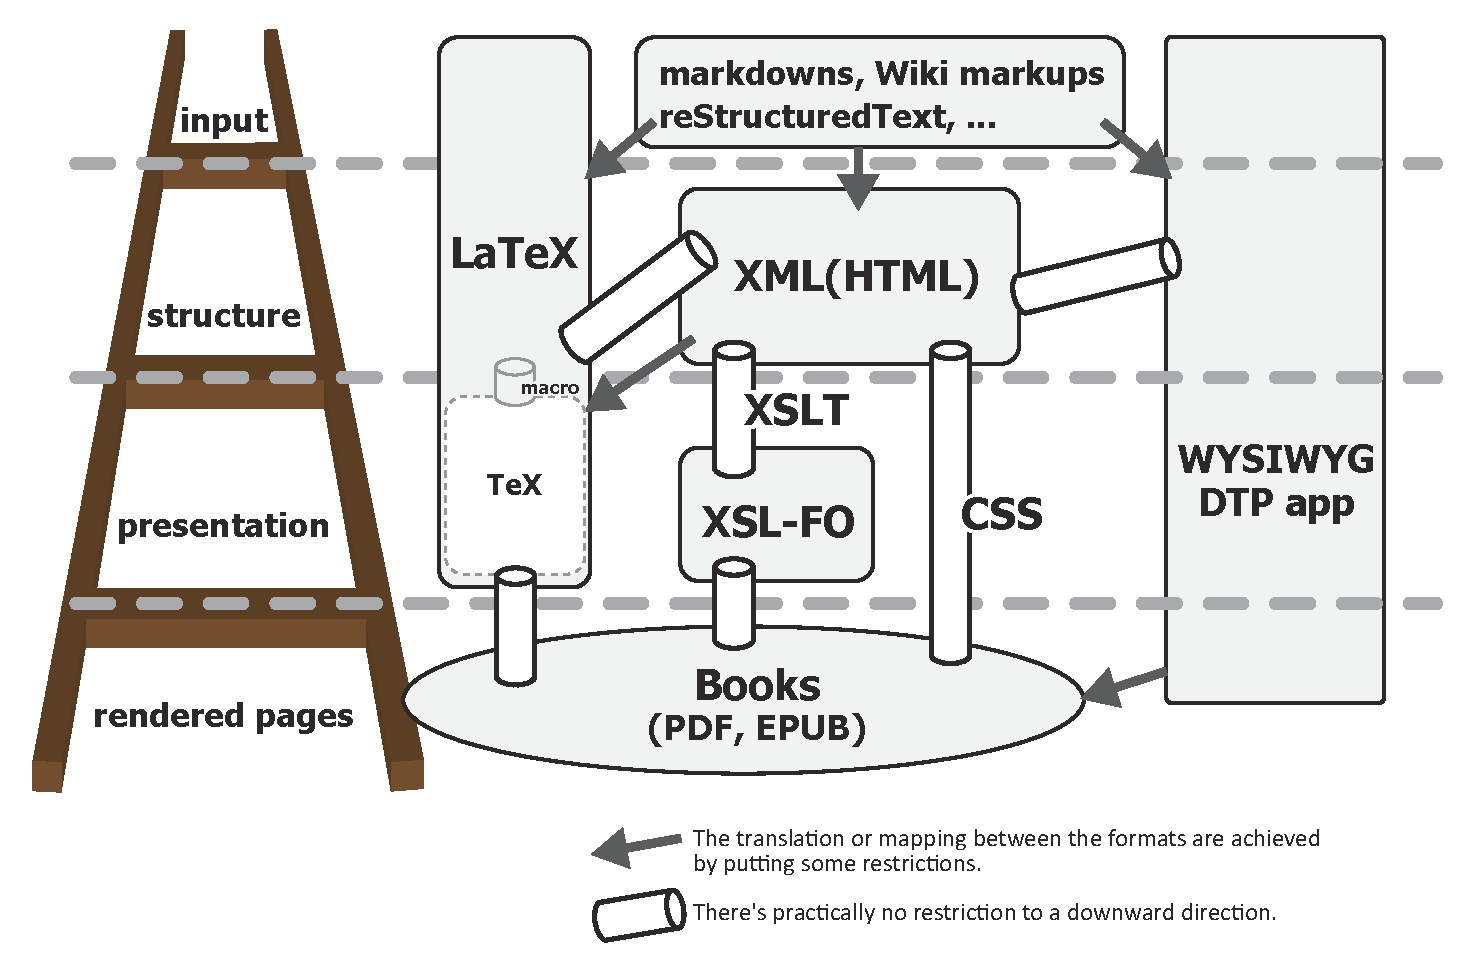
\includegraphics[width=\hsize]{ladder.pdf}
\end{wrapfigure}

{\sffamily キーワード}
\begin{itemize}
\leftskip2em
\item Markdown
\item reStructuredText
\item Re:VIEW
\item XML、xml2tex
\end{itemize}

\end{document}




